Eine relevante Größe für die Beschreibung von Ladungsträgern in Gasen ist die Beweglichkeit $\mu$:

\[v_D = \mu\cdot E \cdot \frac{p_0}{p}  \]

mit dem Gasdruck $p$ und $p_0\approx 1013\,$mbar. $\mu$ ist die Proportionalitätskonstante zwischen
dem elektrischen Feld $E$ und der mittleren Geschwindigkeit $v_D$ des Ladungsträgers, der
sogenannten Driftgeschwindigkeit, die dieser im Feld $E$ erreicht.
\\
Bei Gasgemischen gilt:

\[\frac{1}{\mu_{i^+}} = \sum_{k=1}^n \frac{c_k}{\mu_{i^+_k}}  \]

wobei $c_k$ der Volumenkonzentration des Gases $k$ entspricht und $\mu_{i^+_k}$ der Beweglichkeit
des Ions der Sorte $i$ im Gas $k$.

\begin{figure}[H]
	\centering
	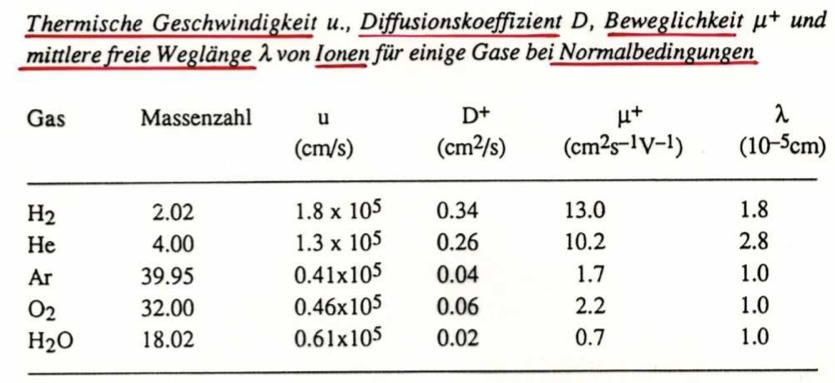
\includegraphics[width=0.5\textwidth]{Fig-03-02.jpg}
\end{figure}

\begin{figure}[H]
	\centering
	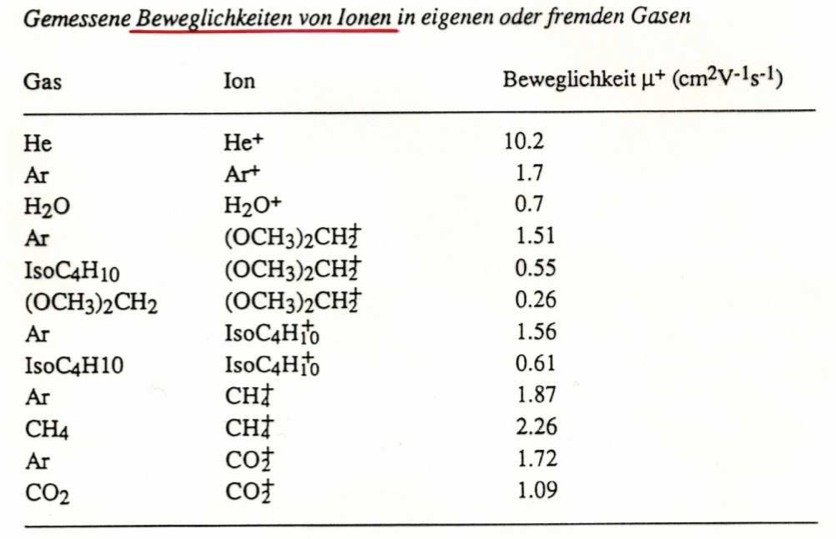
\includegraphics[width=0.5\textwidth]{Fig-03-03.jpg}
\end{figure}

\begin{figure}[H]
	\centering
	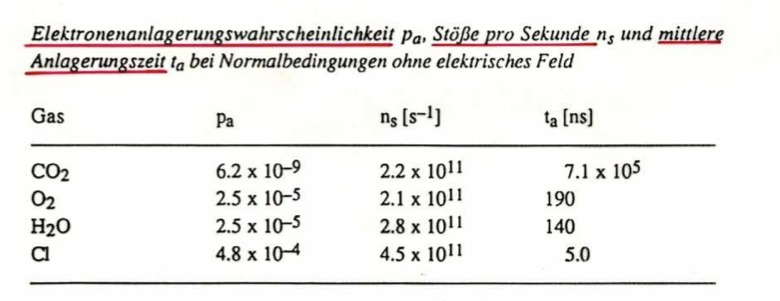
\includegraphics[width=0.5\textwidth]{Fig-03-04.jpg}
\end{figure}

